\chapter{The Future: Ethics, Collaboration, and Frontiers}\label{ch:future}
\begin{center}\small\textit{Powerful tools demand wise hands. The future of AI in software engineering is not just what we can build, but what we should.}\end{center}

\begin{quote}\small\textbf{From zero: no ethics or IP background assumed.} We build from everyday notions of fairness, ownership, and teamwork to the specific tensions AI brings to code, then map open research frontiers. Pictures anchor every idea.\end{quote}

\noindent\fbox{\parbox{\dimexpr\linewidth-2\fboxsep-2\fboxrule}{%
\textbf{Learning Outcomes.} After this chapter you will be able to (1)~name ethical risks of AI-generated code; (2)~explain IP and licensing tensions; (3)~contrast automation, augmentation, and collaboration modes; (4)~sketch human--AI pair-programming patterns; (5)~map current research frontiers and evaluate their maturity.}}
\vspace{0.4em}

% ============================================================
\section{Intuition: Why ``Just Ship It'' Is Not Enough}\label{sec:why-ethics}
An AI assistant can write a sorting routine in seconds. It can also write one that silently leaks user data, copies a GPL-licensed snippet without attribution, or reproduces a biased hiring filter from its training data. Speed without stewardship repeats the oldest failure in software: optimising for \emph{can} while ignoring \emph{should}.

This chapter treats that gap as engineering, not philosophy. For each concern we name the risk, show where it bites in the lifecycle, and give a concrete mitigation a team can adopt next sprint.

% ============================================================
\section{Ethics in AI-Generated Code}\label{sec:ethics}
Four risks dominate practice:

\begin{itemize}[leftmargin=1.2em, itemsep=0.35em]
  \item \textbf{Bias and fairness.} Training data reflect historical decisions --- including biased ones. An AI code generator trained on Stack Overflow may suggest weaker input validation for certain locales, or a ranking model may deprioritise bugs filed by non-native English speakers if their reports use different phrasing.
  \item \textbf{Safety and accountability.} Who is liable when auto-generated code causes an outage or a security breach? The developer who accepted the suggestion, the team that deployed it, or the model provider? Current practice places responsibility on the human committer, which means review obligations do not shrink just because a machine drafted the code.
  \item \textbf{Transparency.} Developers need to know \emph{why} a suggestion was made and \emph{what} sources influenced it. Black-box generation without provenance makes auditing impossible.
  \item \textbf{Environmental and labour costs.} Training large code models consumes significant energy; labelling data for review models relies on human annotators. Ethical adoption weighs these costs against gains.
\end{itemize}

Mitigations that work: diverse evaluation datasets that include under-represented bug types and locales, bias audits on flagged-vs.-accepted warnings across author demographics, mandatory human sign-off on generated security-critical code, and energy budgets in model selection (a smaller distilled model at 95\% of the quality for 10\% of the cost is often the responsible choice).

\begin{center}
\begin{tikzpicture}[font=\scriptsize, >=Stealth, scale=0.88]
  \node[draw, fill=blue!10, rounded corners, minimum width=2.4cm, minimum height=0.85cm, align=center] (data) at (0,0) {Training data\\{\tiny code + reviews}};
  \node[draw, fill=orange!14, rounded corners, minimum width=2.4cm, minimum height=0.85cm, align=center] (model) at (4.0,0) {Code model\\{\tiny LLM / GNN}};
  \node[draw, fill=green!12, rounded corners, minimum width=2.4cm, minimum height=0.85cm, align=center] (gen) at (8.0,0) {Generated code\\{\tiny + suggestion}};
  \node[draw, fill=red!10, rounded corners, minimum width=2.4cm, minimum height=0.85cm, align=center] (harm) at (8.0,-1.6) {Potential harm\\{\tiny bug / bias / leak}};
  \node[draw, fill=violet!12, rounded corners, minimum width=2.4cm, minimum height=0.85cm, align=center] (gate) at (4.0,-1.6) {Guardrails\\{\tiny tests, review, provenance}};
  \node[draw, fill=gray!12, rounded corners, minimum width=2.4cm, minimum height=0.85cm, align=center] (ship) at (0,-1.6) {Shipped code\\{\tiny monitored}};
  \draw[->, thick, blue!60!black] (data) -- (model);
  \draw[->, thick, orange!70!black] (model) -- (gen);
  \draw[->, thick, red!60!black] (gen) -- (harm);
  \draw[->, thick, violet!60!black] (gen) -- (gate);
  \draw[->, thick, violet!60!black] (harm) -- (gate);
  \draw[->, thick, green!50!black] (gate) -- (ship);
  \node[font=\tiny, fill=yellow!10, draw, rounded corners, inner sep=2pt] at (4.0,1.05) {Bias enters here $\to$ guardrails must sit here};
\end{tikzpicture}
\end{center}

% ============================================================
\section{Intellectual Property and Licensing}\label{sec:ip}
Code is intellectual property. When an LLM is trained on public repositories, it may memorise and regurgitate licensed code verbatim. Three tensions follow:

\begin{enumerate}[leftmargin=1.2em, itemsep=0.3em]
  \item \textbf{Licence compliance.} GPL, AGPL, and other copyleft licences require derivative works to carry the same licence. Pasting an AI suggestion that reproduces GPL code into a proprietary codebase can create legal exposure.
  \item \textbf{Attribution.} Many open-source licences (MIT, Apache-2.0) require attribution. If the model strips provenance, the user cannot comply.
  \item \textbf{Ownership of generated code.} Is AI output owned by the user, the model provider, or no one? Jurisdictions differ, and terms of service vary --- teams must read them rather than assume.
\end{enumerate}

Practical hygiene: (i)~enable provenance and licence filters (``block suggestions matching known GPL snippets above 80\% similarity''); (ii)~treat AI output like third-party code --- scan it with a Software Composition Analysis (SCA) tool before merge; (iii)~prefer models trained on permissively licensed data or with opt-out honoured; (iv)~document AI assistance in commit messages for auditability. None of this replaces legal counsel, but it prevents the most common mistakes.

% ============================================================
\section{Human--AI Collaboration: Augmentation, Not Replacement}\label{sec:collab}
Three interaction modes describe how humans and AI share work:

\begin{center}
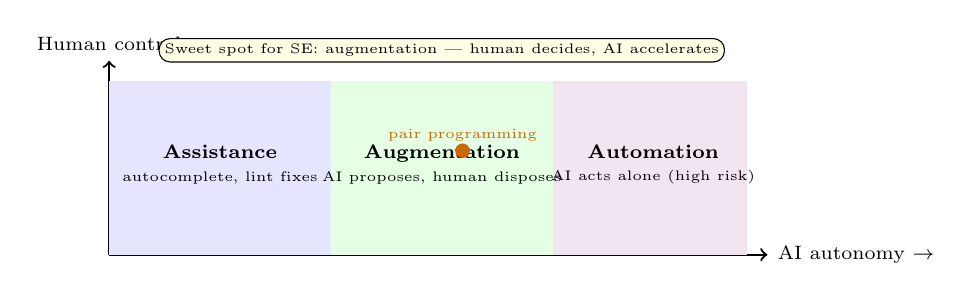
\begin{tikzpicture}[font=\scriptsize, scale=0.88]
  % Automation vs augmentation axis
  \draw[->, thick] (0,0) -- (9.5,0) node[right] {AI autonomy $\to$};
  \draw[->, thick] (0,0) -- (0,2.8) node[above] {Human control};
  % zones
  \fill[blue!10] (0,0) rectangle (3.2,2.5);
  \fill[green!10] (3.2,0) rectangle (6.4,2.5);
  \fill[violet!10] (6.4,0) rectangle (9.2,2.5);
  \node[align=center] at (1.6,1.3) {\textbf{Assistance}\\{\tiny autocomplete, lint fixes}};
  \node[align=center] at (4.8,1.3) {\textbf{Augmentation}\\{\tiny AI proposes, human disposes}};
  \node[align=center] at (7.85,1.3) {\textbf{Automation}\\{\tiny AI acts alone (high risk)}};
  \node[font=\tiny, fill=yellow!10, draw, rounded corners, inner sep=2pt, align=center] at (4.8,2.95) {Sweet spot for SE: augmentation --- human decides, AI accelerates};
  % current practice dot
  \fill[orange!80!black] (5.1,1.5) circle (3pt) node[above, font=\tiny] {pair programming};
\end{tikzpicture}
\end{center}

\textbf{Pair-programming with AI} is the dominant pattern today. The driver (human) states intent, the AI navigator suggests completions, tests, or refactors, and the human accepts, edits, or rejects. Good collaboration design follows three principles: \textbf{initiative balance} (AI suggests, human steers; either can ask ``why?''), \textbf{common ground} (shared view of the codebase, open files, and recent errors), and \textbf{calibrated trust} (show confidence and alternatives, not just one answer).

\begin{center}
\begin{tikzpicture}[font=\scriptsize, >=Stealth, scale=0.86, actor/.style={draw, rounded corners, minimum width=2.2cm, minimum height=1.0cm, align=center}]
  \node[actor, fill=blue!12] (human) at (0,0) {Human\\{\tiny intent, taste, accountability}};
  \node[actor, fill=green!12] (ai) at (5.0,0) {AI assistant\\{\tiny completions, tests, docs}};
  \node[actor, fill=orange!14] (artefact) at (10.0,0) {Shared artefact\\{\tiny code + tests + review}};
  \draw[<->, thick, blue!60!black] (human) -- node[above, font=\tiny, fill=white, inner sep=1pt] {prompt / feedback} (ai);
  \draw[->, thick, green!50!black] (ai) -- node[above, font=\tiny, fill=white, inner sep=1pt] {suggestion + confidence} (artefact);
  \draw[->, thick, orange!70!black] (human) -- node[below, font=\tiny, fill=white, inner sep=1pt] {edit / accept / reject} (artefact);
  % loop back
  \draw[->, thick, dashed, gray!60!black, bend left=18] (artefact.south) to node[below, font=\tiny, fill=white, inner sep=1pt] {test result / review comment} (ai.south);
  \node[draw, fill=yellow!10, rounded corners, font=\tiny, align=left, inner sep=3pt] at (5.0,-1.7) {Context window = open files + diagnostics + chat history;\\trust signal = confidence + alternatives + provenance.};
\end{tikzpicture}
\end{center}

Anti-patterns to avoid: \emph{automation bias} (accepting suggestions without reading them), \emph{deskilling} (novices who never learn to write a test because AI always does), and \emph{accountability drift} (``the AI wrote it'' as an excuse). Mitigate with mandatory reading time for AI diffs, learning-oriented prompts (``explain, don't just fix''), and clear ownership rules.

% ============================================================
\section{Research Frontiers}\label{sec:frontiers}
Where is the field heading? Five frontiers are worth tracking, ordered from ``shipping now'' to ``still speculative.''

\begin{center}
\begin{tikzpicture}[font=\scriptsize, >=Stealth, scale=0.85]
  \foreach \i/\label/\col in {
    1/Repo-level reasoning/blue!12,
    2/Spec-to-code synthesis/green!12,
    3/Self-healing systems/orange!14,
    4/Formal + neural/violet!12,
    5/Agents for SE/gray!14} {
    \pgfmathsetmacro{\x}{(\i-1)*2.45}
    \node[draw, fill=\col, rounded corners, minimum width=2.15cm, minimum height=0.95cm, align=center] (f\i) at (\x,0) {\label};
  }
  \draw[->, thick, blue!60!black] (f1) -- (f2);
  \draw[->, thick, blue!60!black] (f2) -- (f3);
  \draw[->, thick, orange!70!black] (f3) -- (f4);
  \draw[->, thick, violet!60!black] (f4) -- (f5);
  % maturity bar below
  \fill[green!55!black] (0,-1.2) rectangle (4.9,-1.4) node[midway, above, font=\tiny, text=black, yshift=0.55cm] {};
  \fill[orange!60!black] (4.9,-1.2) rectangle (7.35,-1.4);
  \fill[red!55!black] (7.35,-1.2) rectangle (9.8,-1.4);
  \node[font=\tiny] at (2.45,-1.75) {shipping};
  \node[font=\tiny] at (6.15,-1.75) {emerging};
  \node[font=\tiny] at (8.6,-1.75) {speculative};
  \draw[->, thick, gray!60!black] (0,-1.3) -- (9.8,-1.3);
  \node[font=\tiny, text=gray!60!black, align=left] at (5,-2.25) {Repo-level context $\to$ whole-task agents. Maturity falls rightward.};
\end{tikzpicture}
\end{center}

\begin{enumerate}[leftmargin=1.2em, itemsep=0.3em]
  \item \textbf{Repository-level reasoning.} From single-file completion to whole-repo understanding: cross-file references, build graphs, and issue history. Retrieval-augmented generation over the repo is the current workhorse.
  \item \textbf{Specification-to-code synthesis.} Generate implementations from natural-language specs or formal contracts, with verification closing the loop (``generate and prove'').
  \item \textbf{Self-healing systems.} Detect, diagnose, and patch failures autonomously in production, with humans approving patches that touch state or money.
  \item \textbf{Neuro-symbolic SE.} Combine neural generation with symbolic guarantees: type checkers, model checkers, and program analysers as oracles that reject bad generations before a human sees them.
  \item \textbf{Autonomous SE agents.} End-to-end agents that plan (decompose an issue into steps), act (edit, test, observe), and reflect (fix failures) over long horizons --- evaluated on SWE-bench and similar benchmarks. Still brittle on large refactors.
\end{enumerate}

Two evaluation shifts accompany these frontiers: from static benchmarks (HumanEval) to \textbf{interactive, repository-scale} tasks (SWE-bench, Defects4J with CI), and from accuracy alone to \textbf{cost, latency, and regret} (how much human time was actually saved, and at what risk?).

\begin{example}[Provenance check for a generated snippet]\label{ex:provenance}
\begin{lstlisting}[language=Python,caption={Checking a generated snippet against a licence-blocked corpus.},label={lst:provenance}]
import difflib

BLOCKED_SNIPPETS = [
    "def quicksort(arr):\n    if len(arr) <= 1:\n        return arr\n    pivot = arr[len(arr)//2]",  # toy GPL example
]

def max_similarity(generated: str, corpus) -> float:
    return max(difflib.SequenceMatcher(None, generated, s).ratio() for s in corpus)

generated = "def quicksort(arr):\n    if len(arr) <= 1:\n        return arr\n    pivot = arr[len(arr)//2]\n    left = [x for x in arr if x < pivot]"
score = max_similarity(generated, BLOCKED_SNIPPETS)
print(f"max similarity to blocked corpus: {score:.2f}")
if score > 0.80:
    print("BLOCK: too close to copyleft code -- rewrite or attribute")
else:
    print("PASS: no close match")
\end{lstlisting}
\end{example}

% ============================================================
\section{Putting Ethics into Practice: A Checklist}\label{sec:checklist}
Teams can operationalise this chapter with a short pre-merge checklist:

\begin{enumerate}[leftmargin=1.2em, itemsep=0.3em]
  \item \textbf{Provenance check passed?} SCA scan for licence conflicts, similarity to blocked corpus below threshold.
  \item \textbf{Bias audit clean?} Acceptance rate of AI suggestions does not differ by author locale or team at $p<0.05$.
  \item \textbf{Human sign-off present?} Every AI-generated change to auth, payments, or data handling has a human reviewer who can explain it.
  \item \textbf{Energy budget respected?} Model choice justified against a smaller baseline; batch inference where possible.
\end{enumerate}

A second listing extends provenance to embeddings for scale:

\begin{lstlisting}[language=Python,caption={Scaled provenance with TF-IDF nearest neighbour.},label={lst:provenance2}]
from sklearn.feature_extraction.text import TfidfVectorizer
from sklearn.metrics.pairwise import cosine_similarity

corpus = ["def quicksort(arr):\n    if len(arr)<=1: return arr", "def mergesort(a):\n    ..."]
gen = "def quicksort(arr):\n    if len(arr)<=1: return arr\n    pivot=arr[0]"
vec = TfidfVectorizer().fit(corpus + [gen])
M = vec.transform(corpus + [gen])
sims = cosine_similarity(M[-1], M[:-1]).flatten()
print("max cosine:", sims.max(), "closest idx:", sims.argmax())
if sims.max() > 0.80:
    print("flag for manual licence review")
\end{lstlisting}

% ============================================================
\section{Chapter Summary}\label{sec:future-summary}
Powerful code models amplify both capability and responsibility. Ethics demands guardrails for bias, safety, transparency, and cost; IP demands provenance and licence hygiene; collaboration demands augmentation designs where humans decide and AI accelerates. The frontier moves from file-level completion to repo-level agents with symbolic checks --- and the measure of progress will be human time saved without regret.

% ============================================================
\section{Exercises}\label{sec:future-ex}
\begin{enumerate}[label=E8.\arabic*, leftmargin=*, itemsep=0.75em]
  \item \textbf{Bias audit.} Your defect ranker flags bugs from one team 2$\times$ more often than another at the same threshold. Propose a metric to detect this, a hypothesis for why it happens (training data? wording?), and a mitigation that preserves overall recall.
  \item \textbf{Licence hygiene.} A generated 20-line function matches a GPL file at 85\% similarity. List three lawful options for the team and one that is not. When would you choose rewriting over attribution?
  \item \textbf{Collaboration design.} Sketch a pair-programming interaction where the AI suggests a fix with low confidence and two alternatives. What UI elements convey confidence and provenance without overwhelming the developer?
  \item \textbf{Frontier maturity.} Place ``self-healing patch for a null dereference in a Java microservice'' on the maturity bar of Fig.~2. Justify with a concrete benchmark (Defects4J, SWE-bench) and state what would promote it from emerging to shipping.
  \item \textbf{Provenance extension.} Extend Listing~\ref{lst:provenance} to check against 100 snippets efficiently (hint: MinHash or embedding nearest-neighbour) and to report the closest match with its licence. Discuss false positives from boilerplate (e.g., getters).
\end{enumerate}
% End of Chapter 8
